\documentclass{article}
\usepackage[utf8]{inputenc}  
\usepackage[T1]{fontenc}     
\usepackage{tikz}
\usetikzlibrary{shapes,positioning,arrows,calc}
\usetikzlibrary{decorations.pathreplacing}

\begin{document}

% tri : exemple

% tour 1

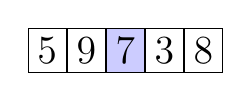
\begin{tikzpicture}
\node [font=\sffamily\Large\bfseries, draw, anchor=center] (first) {$5$};
\node [font=\sffamily\Large\bfseries, draw, anchor=center, right=0cm of first] (second) {$9$};
\node [fill=blue!20, font=\sffamily\Large\bfseries, draw, anchor=center, right=0cm of second] (third) {$7$};
\node [font=\sffamily\Large\bfseries, draw, anchor=center, right=0cm of third] (fourth) {$3$};
\node [font=\sffamily\Large\bfseries, draw, anchor=center, right=0cm of fourth] (fifth) {$8$};
\end{tikzpicture}

\vspace{0.25cm}

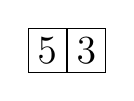
\begin{tikzpicture}
\node [font=\sffamily\Large\bfseries, draw, anchor=center] (first) {$5$};
\node [font=\sffamily\Large\bfseries, draw, anchor=center, right=0cm of first] (second) {$3$};
\end{tikzpicture}
\hspace{0.1cm}
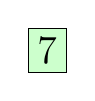
\begin{tikzpicture}
\node [fill=green!20, font=\sffamily\Large\bfseries, draw, anchor=center] (first) {$7$};
\end{tikzpicture}
\hspace{0.1cm}
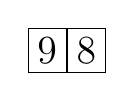
\begin{tikzpicture}
\node [font=\sffamily\Large\bfseries, draw, anchor=center] (first) {$9$};
\node [font=\sffamily\Large\bfseries, draw, anchor=center, right=0cm of first] (second) {$8$};
\end{tikzpicture}

% tour 2

\vspace{1cm}

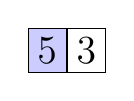
\begin{tikzpicture}
\node [fill=blue!20, font=\sffamily\Large\bfseries, draw, anchor=center] (first) {$5$};
\node [font=\sffamily\Large\bfseries, draw, anchor=center, right=0cm of first] (second) {$3$};
\end{tikzpicture}
\hspace{0.1cm}
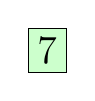
\begin{tikzpicture}
\node [fill=green!20, font=\sffamily\Large\bfseries, draw, anchor=center] (first) {$7$};
\end{tikzpicture}
\hspace{0.1cm}
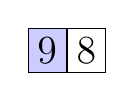
\begin{tikzpicture}
\node [fill=blue!20, font=\sffamily\Large\bfseries, draw, anchor=center] (first) {$9$};
\node [font=\sffamily\Large\bfseries, draw, anchor=center, right=0cm of first] (second) {$8$};
\end{tikzpicture}

\vspace{0.25cm}


\begin{tikzpicture}
\node [font=\sffamily\Large\bfseries, draw, anchor=center] (first) {$3$};
\end{tikzpicture}
\hspace{0.1cm}
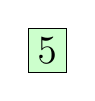
\begin{tikzpicture}
\node [fill=green!20, font=\sffamily\Large\bfseries, draw, anchor=center] (first) {$5$};
\end{tikzpicture}
\hspace{0.1cm}
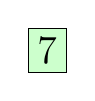
\begin{tikzpicture}
\node [fill=green!20, font=\sffamily\Large\bfseries, draw, anchor=center] (first) {$7$};
\end{tikzpicture}
\hspace{0.1cm}

\begin{tikzpicture}
\node [font=\sffamily\Large\bfseries, draw, anchor=center] (first) {$8$};
\end{tikzpicture}
\hspace{0.1cm}
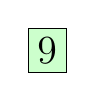
\begin{tikzpicture}
\node [fill=green!20, font=\sffamily\Large\bfseries, draw, anchor=center] (first) {$9$};
\end{tikzpicture}


\vspace{1cm}

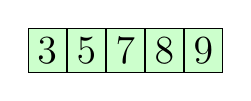
\begin{tikzpicture}
\node [fill=green!20, font=\sffamily\Large\bfseries, draw, anchor=center] (first) {$3$};
\node [fill=green!20, font=\sffamily\Large\bfseries, draw, anchor=center, right=0cm of first] (second) {$5$};
\node [fill=green!20, font=\sffamily\Large\bfseries, draw, anchor=center, right=0cm of second] (third) {$7$};
\node [fill=green!20, font=\sffamily\Large\bfseries, draw, anchor=center, right=0cm of third] (fourth) {$8$};
\node [fill=green!20, font=\sffamily\Large\bfseries, draw, anchor=center, right=0cm of fourth] (fifth) {$9$};
\end{tikzpicture}


\end{document}